\documentclass[a4paper]{article}
\usepackage[utf8]{inputenc}
\usepackage[czech]{babel}
\usepackage[T1]{fontenc}

\usepackage[pdftex]{graphicx}
\usepackage{ifpdf}
\usepackage{hyperref}

\title{gScrabble -- Uživatelská příručka}

\author{Ondrej Profant}

\date{\today}

\ifpdf
\hypersetup{
	pdfauthor={Ondrej Profant},
	pdftitle={gScrabble -- Uzivatelská prirucka},
}
\fi
\begin{document}

\tableofcontents	


\section{Úvod}
gScrabble je implementací klasické deskové hry Scrabble, která svou pomáhá rozvíjet slovní zásobu již 50 let. Snahou autora bylo vytvořit jednoduchý program, který zvládne obsluhovat každý a bude dostupný pro co nejvíce OS. Program je volně dostupný ke stažení a k jakémukoliv používání (viz Licence).

Pokud by se vám program i přesto nelíbil, tak můžete vyzkoušet konkurenci -- např. \href{http://people.csail.mit.edu/jasonkb/quackle/}{Quackle} (Qt).
\section{Licence}
Program je pod GNU General Public License, která zajišťuje uživateli právo modifkovat, kopírovat a dále šířit zdrojový kód. Plné znění naleznete přiložené u programu nebo na adresách:
\href{http://www.gnugpl.cz/}{gnugpl.cz} (česky, neoficiální překlad) a \href{http://www.gnu.org/licenses/gpl-3.0.txt}{gnu.org/licenses/gpl-3.0.txt} (anglicky, oficiální verze).

\section{Instalace}
Program není třeba instalovat. Stačí ho spustit v Mono frameworku, popřípadě v .NET frameworku. Pro různé operační systémy a architektury procesory (x86, x64) je stejný binární soubor.
Jsou dvě možnosti spuštění:
\begin{itemize}
\item[Terminál]: \texttt{\$: mono gscrabble.exe} 
\item[Grafické rozhraní]: Pravým myšítkem klikneme na gscrabble.exe a ve vlastnostech ověříme, že parametr "spustit s..." je nastaven na mono či .NET. Poté již spouštíme normálně dvojklikem (levým myšítkem).
\end{itemize}
\subsection{Potřebné knihovny}
Program potřebuje již zmíněné \texttt{mono} ve verzi 2.10 a novější. Dále potřebuje GTK\# ve verzi 2.12 a novější. Oboje je ke stažení na: \href{http://www.go-mono.com/mono-downloads}{go-mono.com}. Nejnovější informace o podporovaných a testovaných systémech jsou v souboru README.

\section{Slovník}
Program svůj interní slovník nahrává při každém spuštění z prostého textového souboru. V tom jsou jednotlivá slova oddělená čárkou a mezerou, takto:
\texttt{do, don, dort, dost, dosti, \ldots{}} 

Můžete do něj dopsat či z něj vymazat jakékoliv slovo ve vašem oblíbeném textovém editoru\footnote{Windows: Notepad, Pspad; Linux: Gedit, Geany, Leafpad; \ldots{}} (jen vždy uložte jako prostý text s kodováním UTF-8). 

\subsection{Český}
Volně ke stažení je slovník Blex-Klasik, který obsahuje 34 263 délky 2--5. Najdete ho na \href{http://scrabble.hrejsi.cz/pravidla/blex.htm}{scrabble.hrejsi.cz}.

\section{Ovládání programu}
Program se ovládá výhradně přes grafické rozhraní. Cílem autora byla maximální jednoduchost.

\subsection{Konfigurační okno}
\begin{center}
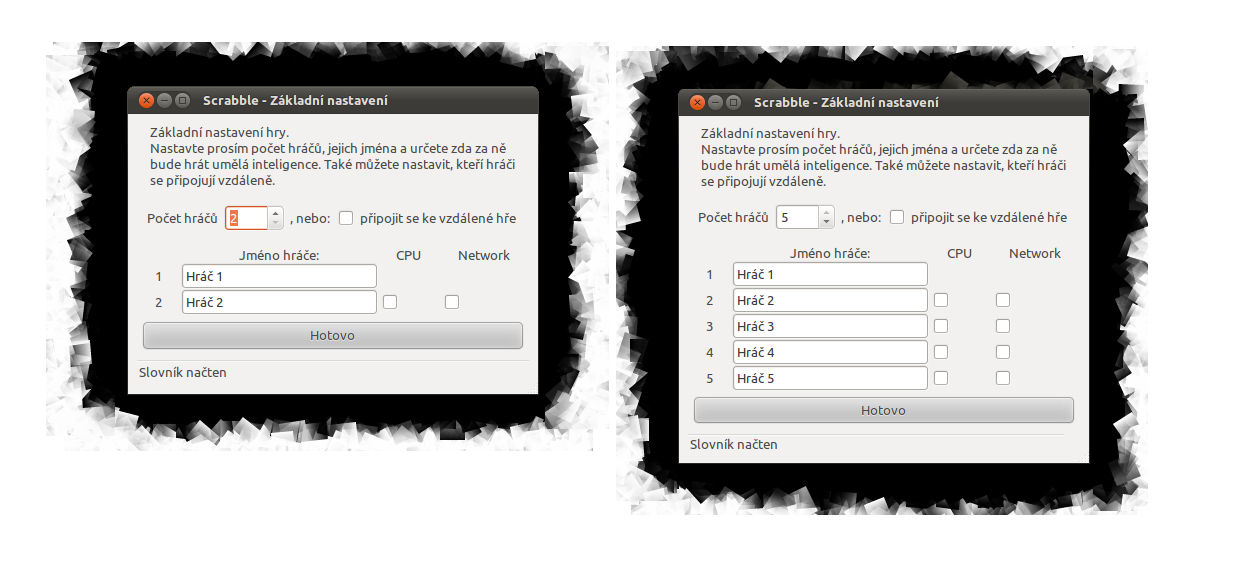
\includegraphics[scale=1.2]{pic/configWin.png}
Obrázek 1: Konfigurační okno
\end{center}
V konfiguračním okně můžete nastavit počet hráčů (tabulka dole se dynamicky mění). U každého hráče můžete zvolit jméno a dále zaškrtnou zda za něj má hrát počítač (CPU), či zda to bude hráč připojený přes síť. V druhém případě se následně ještě objeví sloupec do kterého vyplníte IP adresu vzdáleného hráče. 

Pokud zaškrtnete volbu \texttt{připojit se ke vzdálené hře}, tak hra počká, až bude zavolána z jiného počítače (kde vyplníte IP adresu, jak bylo popsáno v minulém bodě). Toto spojení (zvláště poprvé) může chvíli trvat, mějte strpení.

\subsection{Hlavní okno hry}
Hlavnímu oknu hry dominuje hrací deska, nahoře je klasická nabídka (na MacOS a Ubuntu bude na místě, kam jí umisťuje systém), dole jsou další informace o hře -- váš zásobník kamenů, možnosti tahu a tabulka s výsledky. Zcela dole se nachází stavový řádek.

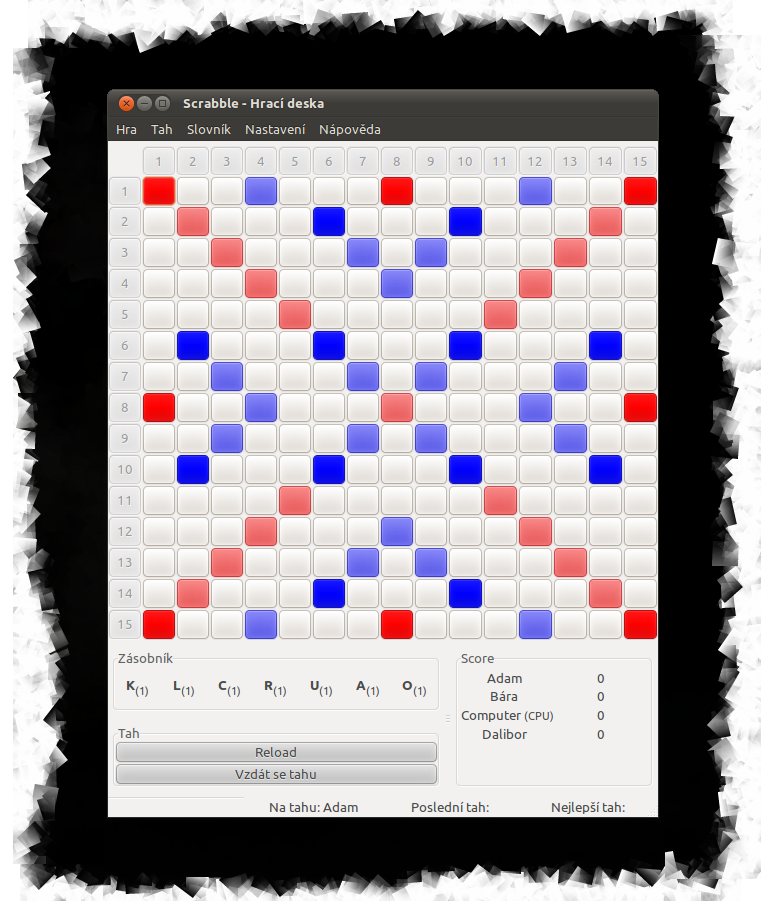
\includegraphics[scale=1]{pic/mainWindow.png}

Pokud jste na tahu, tak se vám po kliknutí na políčko na hracím plánu objeví dialog pro vložení slova. Kliknout musíte vždycky na počáteční pozici nového slova. Klávesou \texttt{Esc} tento dialog zrušíte, klávesou \texttt{Enter} potvrdíte, pokud zaškrtnete down, tak slovo bude položeno vertikálně (zhora dolu).

V případě, že hraje více hráčů u jednoho počítače, tak se před zahájením tahu vždy objeví obrazovka, která vám oznámí kdo hraje.

Nejdůležitější položkou v nabídce je pravděpodobně slovník, která umožňuje ověřovat přítomnost slov ve slovníku (klávesová zkratka \texttt{F5}), přidávat slova do slovníku (\texttt{ctrl+i}), popřípadě nahrát celý nový slovník.

\section{Multiplayer}
\section{Odkazy}
\begin{itemize}
\item \href{http://github.com/Kedrigern/scrabble}{Tento program na github.com} - zde také seženete autora
\item \href{http://scrabble.hrejsi.cz/pravidla/}{Pravidla Scrabble (cs)}
\end{itemize}
\end{document}
